\documentclass{article}

% Paquetes comunes
\usepackage[utf8]{inputenc}
\usepackage[T1]{fontenc}
\usepackage[spanish]{babel}
\usepackage{amsmath, amssymb}
\usepackage{graphicx}
\usepackage{float}
\usepackage{geometry}
\usepackage{hyperref}
\usepackage{fancyhdr}
\usepackage{textcomp}
\usepackage{circuitikz}
% Saltar entre párrafos - sin sangrías
\usepackage{parskip}

% Márgenes
\geometry{a4paper, margin=2.5cm}

% Encabezado y pie de página
\pagestyle{fancy}
\fancyhf{}
\fancyhead[L]{\textbf{Tarea 3} - Tomas Infante}
\fancyhead[R]{IEE2513}
\fancyfoot[C]{\thepage}

\title{Tarea 3}
\author{Tomas Infante}
\date{\today}
\begin{document}
\begin{figure}[H]
    \centering
    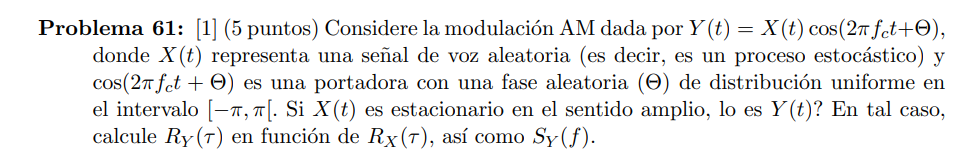
\includegraphics[width=1\textwidth]{Problema_61.png}
    \label{Problema_61}
\end{figure}
Para que \(Y(t)\) sea ESA debe cumplir que:
\begin{enumerate}
    \item \(E\left[Y(t)\right]\) es constante
    \item \(R_Y(t_1,t_2)\) depende solo de \(\tau = t_2-t_1\)
\end{enumerate}
Calculamos primero la esperanza de \(Y(t)\)
\[
E\left[Y(t)\right] = E\left[X(t)\cos(2\pi f_c t + \Theta)\right]
\]
Como \(X(t)\) es independiente \(\Theta\) (Son procesos nacidos de distintas fuentes, por lo que no hay dependencia aparente) tenemos que:
\[
E\left[Y(t)\right] = E\left[X(t)\right]E\left[\cos(2\pi f_c t + \Theta)\right]
\]
Pero:
\[
E\left[\cos(2\pi f_c t + \Theta)\right] = \frac{1}{2 \pi}\int_{-\pi}^{\pi}\cos(2\pi f_c t + \Theta)\,d\Theta
\]
\[
= \frac{1}{2 \pi}\left[\sin(2\pi f_c t + \Theta)\right]_{-\pi}^{\pi}
\]
\[
= \frac{1}{2 \pi}\left[\sin(2\pi f_c t + \pi)- \sin(2\pi f_c t - \pi)\right]
\]
Sabemos que \(\sin(a \pm \pi) = -\sin(a)\). Por lo tanto:
\[
= \frac{1}{2 \pi}\left[-\sin(2\pi f_c t)- (-\sin(2\pi f_c t))\right] = 0
\]
\[
E\left[\cos(2\pi f_c t + \Theta)\right] = 0
\]
Lo que implica que:
\[
E\left[Y(t)\right] = E\left[X(t)\right]E\left[\cos(2\pi f_c t + \Theta)\right] = 0
\]
Es decir, \(E\left[Y(t)\right]\) es una constante. Verificamos ahora el criterio de \(R_{Y}(t_1,t_2)\).
\[
R_Y(t_1,t_2) = E\left[Y(t_1)Y(t_2)\right]
\]
\[
R_Y(t_1,t_2)= E\left[X(t_1)\cos(2\pi f_c t_1 + \Theta)X(t_2)\cos(2\pi f_c t_2 + \Theta)\right]
\]
Dado que \(X(t)\) es independiente de \(\Theta\) podemos separa las esperanzas.
\[
R_Y(t_1,t_2)= E\left[X(t_1)X(t_2)\right]\cdot E\left[\cos(2\pi f_c t_1 + \Theta)\cos(2\pi f_c t_2 + \Theta)\right]
\]
Como \(X(t)\) es ESA tenemos que \(E\left[X(t_1)X(t_2)\right] = R_X(t_2-t_1)\). Solo tenemos que resolver:
\[
E\left[\cos(2\pi f_c t_1 + \Theta)\cos(2\pi f_c t_2 + \Theta)\right]
\]
Recordamos que:
\[
\cos(a)\cos(b)= \frac{1}{2}\left[\cos(a-b)+\cos(a+b)\right]
\]
Llegamos a:
\[
E\left[\frac{1}{2}\left[\cos(2\pi f_c t_1 + \Theta-(2\pi f_c t_2 + \Theta))+\cos(2\pi f_c t_1 + \Theta+2\pi f_c t_2 + \Theta)\right]\right]
\]
\[
E\left[\frac{1}{2}\left[\cos(2\pi f_c (t_1-t_2))+\cos(2\pi f_c (t_1+t_2) + 2\Theta)\right]\right]
\]
La epseranza de la suma es la suma de las esperanzas.
\[
\frac{1}{2}E\left[\cos(2\pi f_c (t_1-t_2))\right] + \frac{1}{2}E\left[\cos(2\pi f_c (t_1+t_2) + 2\Theta)\right]
\]
\[
\frac{1}{2}E\left[\cos(2\pi f_c (t_1+t_2) + 2\Theta)\right] = 0
\]
\[
\frac{1}{2}E\left[\cos(2\pi f_c (t_1-t_2))\right] = \frac{1}{2}\cos(2\pi f_c (t_1-t_2))
\]
Como \(\cos(a)=\cos(-a)\):
\[
\frac{1}{2}\cos(2\pi f_c (t_1-t_2)) = \frac{1}{2}\cos(2\pi f_c (t_2-t_1))
\]
Por lo tanto:
\[
R_Y(t_1,t_2)= R_X(t_2-t_1)\cdot\frac{1}{2}\cos(2\pi f_c (t_2-t_1))
\]
Es decir \(R_Y(t_1,t_2)\) depende solo de \(\tau = t_2-t_1\). Como \(Y(t)\) cumple ambas condiciones para ser ESA decimos que \(Y(t)\) es ESA.
\[
R_Y(\tau) = \frac{1}{2}R_X(\tau)\cos(2\pi f_c \tau)
\]
\[
S_Y(f) =\frac{1}{2} \mathcal{F} \left\{R_X(\tau)\cos(2\pi f_c \tau)\right\}
\]
Sabemos que:
\[
\mathcal{F} \left\{\cos(2\pi f_c \tau)\right\} = \frac{1}{2}\left[\delta(f-f_c)+\delta(f+f_c)\right]
\]
Y que:
\[
\mathcal{F} \left\{R_X(\tau)\right\} = S_X(f)
\]
Por lo tanto:
\[
S_Y(f) =\frac{1}{2} \mathcal{F} \left\{R_X(\tau)\cos(2\pi f_c \tau)\right\} =\frac{1}{2} \int_{-\infty}^{\infty}S_X(f-\sigma)\frac{1}{2}\left[\delta(\sigma-f_c)+\delta(\sigma+f_c)\right]\, d\sigma
\]
\[
S_Y(f) = \frac{1}{4}\left[S_{X}(f-f_c)+S_{X}(f+f_c)\right]
\]
\begin{figure}[H]
    \centering
    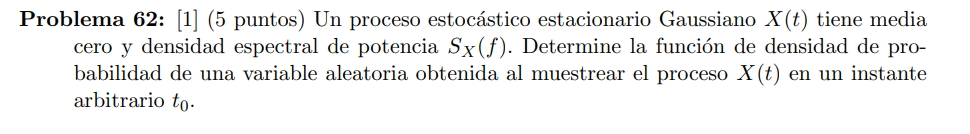
\includegraphics[width=1\textwidth]{Problema_62.png}
    \label{Problema_62}
\end{figure}
Como es un proceso estocastico estacionario Gaussiano se cumple que en cada intante de tiempo, digamos \(t_0\)
\[
X_0 = X(t_0)\thicksim \mathcal{N}(\mu_X,\sigma_X^{2})
\]
Como no dicen que es estacionario de media \(0\) samemos automaricamente que \(\mu_X=0\). Por lo tanto:
\[
X(t_0)\thicksim \mathcal{N}(0,\sigma_X^{2})
\]
Sabemos que:
\[
\sigma_X^{2}= Var(X(t_0)) = E\left[X(t_0)^{2}\right]-\mu_X^{2}
\]
Es decir:
\[
\sigma_X^{2}= E\left[X(t_0)X(t_0)\right]-0
\]
Como \(X(t)\) es ESA tenemos que:
\[
E\left[X(t_0)X(t_0)\right] = R_X(0)
\]
Entonces:
\[
\sigma_X^{2}= R_X(0)
\]
Recordando que:
\[
\mathcal{F}\left\{R_X(\tau)\right\} = S_X(f)
\]
Es decir:
\[
\mathcal{F}^{-1}\left\{S_X(f)\right\} = R_X(\tau)
\]
\[
\int_{-\infty}^{\infty}S_X(f)e^{j2\pi f \tau}\, df = R_X(\tau)
\]
Si tomamos \(\tau = 0\) tenemos:
\[
\int_{-\infty}^{\infty}S_X(f)\,df= R_X(0)
\]
Por lo tanto:
\[
\sigma_X^{2}= R_X(0) = \int_{-\infty}^{\infty}S_X(f)\,df
\]
La densidad de probabilidad de una distribucion gaussiana es:
\[
f_X(x) = \frac{1}{\sqrt{2\pi \sigma^{2}}}e^{-\frac{1}{2}\left(\frac{x-\mu}{\sigma}\right)^{2}}
\]
Para nuestro caso tenemos:
\[
f_{X(t_0)}(x) = \frac{1}{\sqrt{2\pi \int_{-\infty}^{\infty}S_X(f)\,df}}\text{exp}\left(-\frac{x^{2}}{2\int_{-\infty}^{\infty}S_X(f)\,df}\right)
\]
\begin{figure}[H]
    \centering
    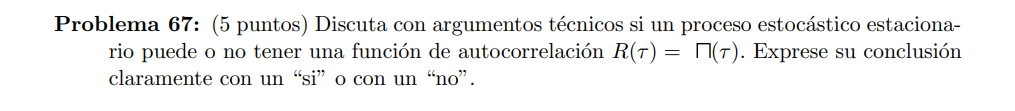
\includegraphics[width=1\textwidth]{Problema_67.png}
    \label{Problema_67}
\end{figure}
Para que un proceso estacionario tenga \(R(\tau)=\sqcap (\tau)\) este proceso debe ser al menos ESA. Y el problema es que si \(\sqcap(\tau)\) fuera la funcion de autocorelacion de un P.E ESA. 
Este deberia generar una densidad espectral de potencia que cumpla, al menos que:
\[
S(f)\geq 0 \quad \forall f
\]
Cosa que no cumpliria \(R(\tau)=\sqcap(\tau)\) ya que:
\[
S(f) = \mathcal{F} \left\{\sqcap(\tau)\right\} = \text{sinc}(f)
\]
El cual no cumple que es mayor a cero para todo \(f\). Es por lo anterior que no puede existir un proceso estacionario con \(R(\tau)=\sqcap(\tau)\) que sea ESA. 
Y por consiguiente tampoco existe un P.E estacionario con \(R(\tau)=\sqcap(\tau)\).
\begin{figure}[H]
    \centering
    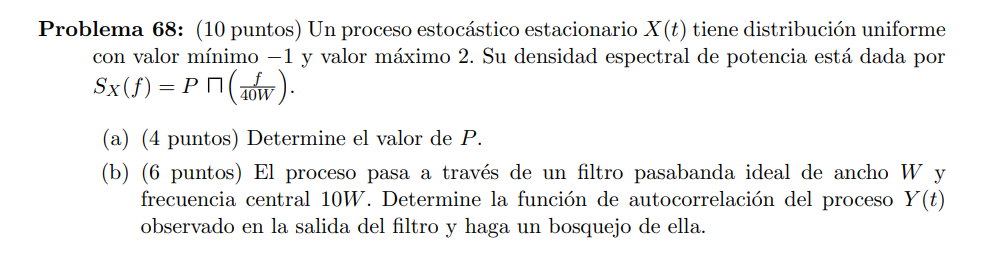
\includegraphics[width=1\textwidth]{Problema_68.png}
    \label{Problema_68}
\end{figure}
\subsection*{\small a)}
Tenemos que por ser estacionario \(\mu_X\) es constante y \(\sigma_X^{2}\) tambien, y sabemos que para una distribucion uniforme son:
\[
\mu_X = \frac{-1+2}{2}=0.5 \quad \quad \sigma_X^{2}=\frac{(2-(-1))^2}{12}=0.75
\]
Por otro lado sabemos que:
\[
E\left[X(t_0)^{2}\right]=\sigma_X^{2}+\mu_X^{2}
\]
\[
E\left[X(t_0)X(t_0)\right]= 0.75 + (0.5)^{2}
\]
Como \(X(t)\) es estacionario tenemos que \(E\left[X(t_0)X(t_0)\right]=R_X(0)\). Por lo tanto:
\[
R_X(0)= 0.75 + (0.5)^{2} = 1
\]
Sabemos por el problema 62. Que:
\[
R_X(0)=\int_{-\infty}^{\infty}S_X(f)\, df
\]
En nuestro caso eso implica que:
\[
1 = \int_{-\infty}^{\infty}P \sqcap\left(\frac{f}{40W}\right)\, df
\]
La funcion \(\sqcap\left(\frac{f}{40W}\right)\) vale \(1\) cuando \(|f|\leq 20W\). Entonces la integral se reduce a:
\[
1 = \int_{-20W}^{20W}P\, df
\]
\[
1 = 40WP \quad \longrightarrow \quad P = \frac{1}{40W}
\]
\subsection*{\small b)}
Como el sistema es LTI. Tenemos que:
\[
S_Y(f)=|H(f)|^{2}S_X(f)
\]
Donde:
\[
H(f)=
\begin{cases}
1, & 10W-\dfrac{W}{2} \le |f| \le 10W+\dfrac{W}{2} \\
0, & \text{en otro caso}
\end{cases}
\]
Entonces:
\[
|H(f)|^{2}=
\begin{cases}
1, & 10W-\dfrac{W}{2} \le |f| \le 10W+\dfrac{W}{2} \\
0, & \text{en otro caso}
\end{cases}
\]
Como \(S_X(f)\) vale \(\frac{1}{40W}\) en ese intervalo, tenemos que:
\[
S_Y(f)=
\begin{cases}
\frac{1}{40W} , & 10W-\dfrac{W}{2} \le |f| \le 10W+\dfrac{W}{2} \\
0, & \text{en otro caso}
\end{cases}
\]
Es decir:
\[
S_Y(f) =\frac{1}{40W}\left[\sqcap\left(\frac{f-10W}{W}\right)+\sqcap\left(\frac{f+10W}{W}\right)\right] 
\]
Sabemos que:
\[
R_Y(\tau)=\mathcal{F}^{-1}\left\{S_Y(f)\right\} 
\]
Y tambien sabemos que:
\[
\mathcal{F}^{-1}\left\{\sqcap\left(\frac{f-f_c}{W}\right)\right\}=W\text{sinc}\left(W\tau\right)e^{j2\pi f_c \tau} 
\]
Por lo tanto:
\[
=\mathcal{F}^{-1}\left\{S_Y(f)\right\} = \mathcal{F}^{-1}\left\{\frac{1}{40W}\left[\sqcap\left(\frac{f-10W}{W}\right)+\sqcap\left(\frac{f+10W}{W}\right)\right] \right\}
\]
\[
=\frac{1}{40W}\mathcal{F}^{-1}\left\{\sqcap\left(\frac{f-10W}{W}\right)\right\} +\frac{1}{40W}\mathcal{F}^{-1}\left\{\sqcap\left(\frac{f+10W}{W}\right)\right\}
\]
\[
=\frac{1}{40W}W\text{sinc}\left(W\tau\right)e^{j2\pi 10W \tau} + \frac{1}{40W}W\text{sinc}\left(W\tau\right)e^{-j2\pi 10W \tau}
\]
Reordenamos:
\[
=\frac{1}{20}\text{sinc}\left(W\tau\right)\left[\frac{e^{j2\pi 10W \tau} + e^{-j2\pi 10W \tau}}{2}\right]
\]
\[
R_Y(\tau)=\frac{1}{20}\text{sinc}\left(W\tau\right)\cos(20\pi W \tau)
\]
Graficamos para \(W=0.1\) asi logramos ver el efecto:
\begin{figure}[H]
    \centering
    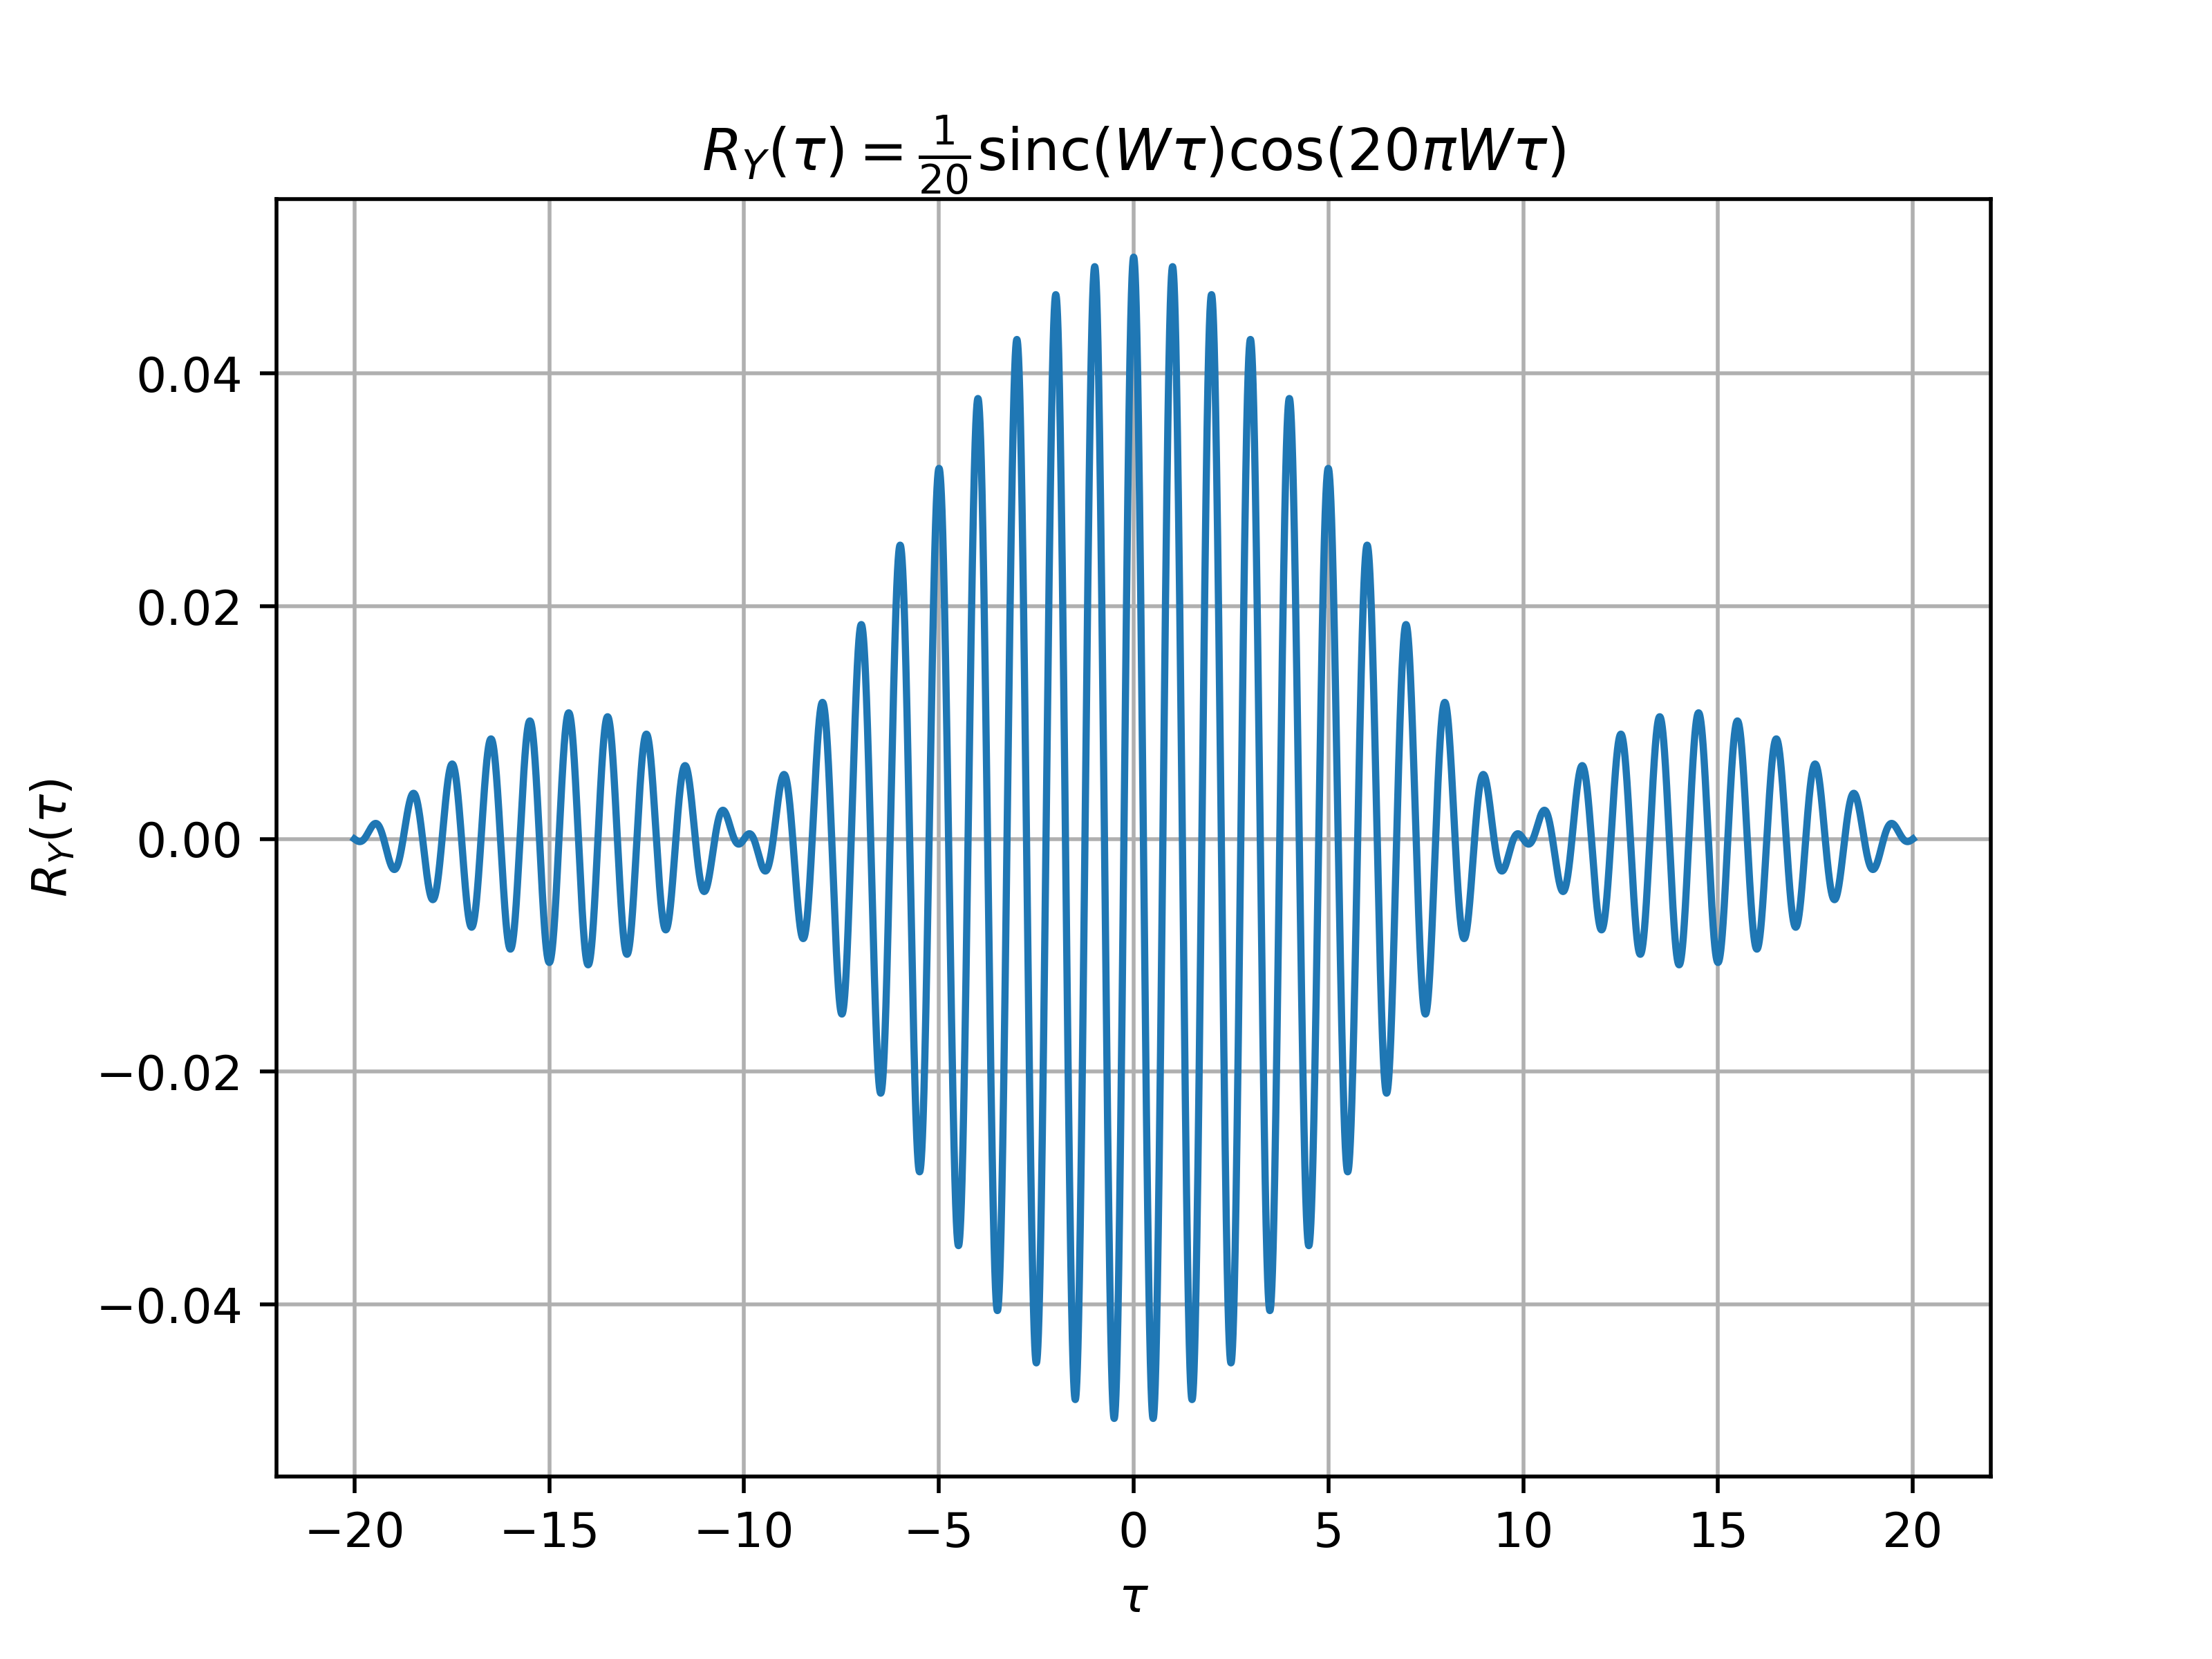
\includegraphics[width=0.7\textwidth]{Grafico_1.png}
    \label{Grafico_1}
\end{figure}
\begin{figure}[H]
    \centering
    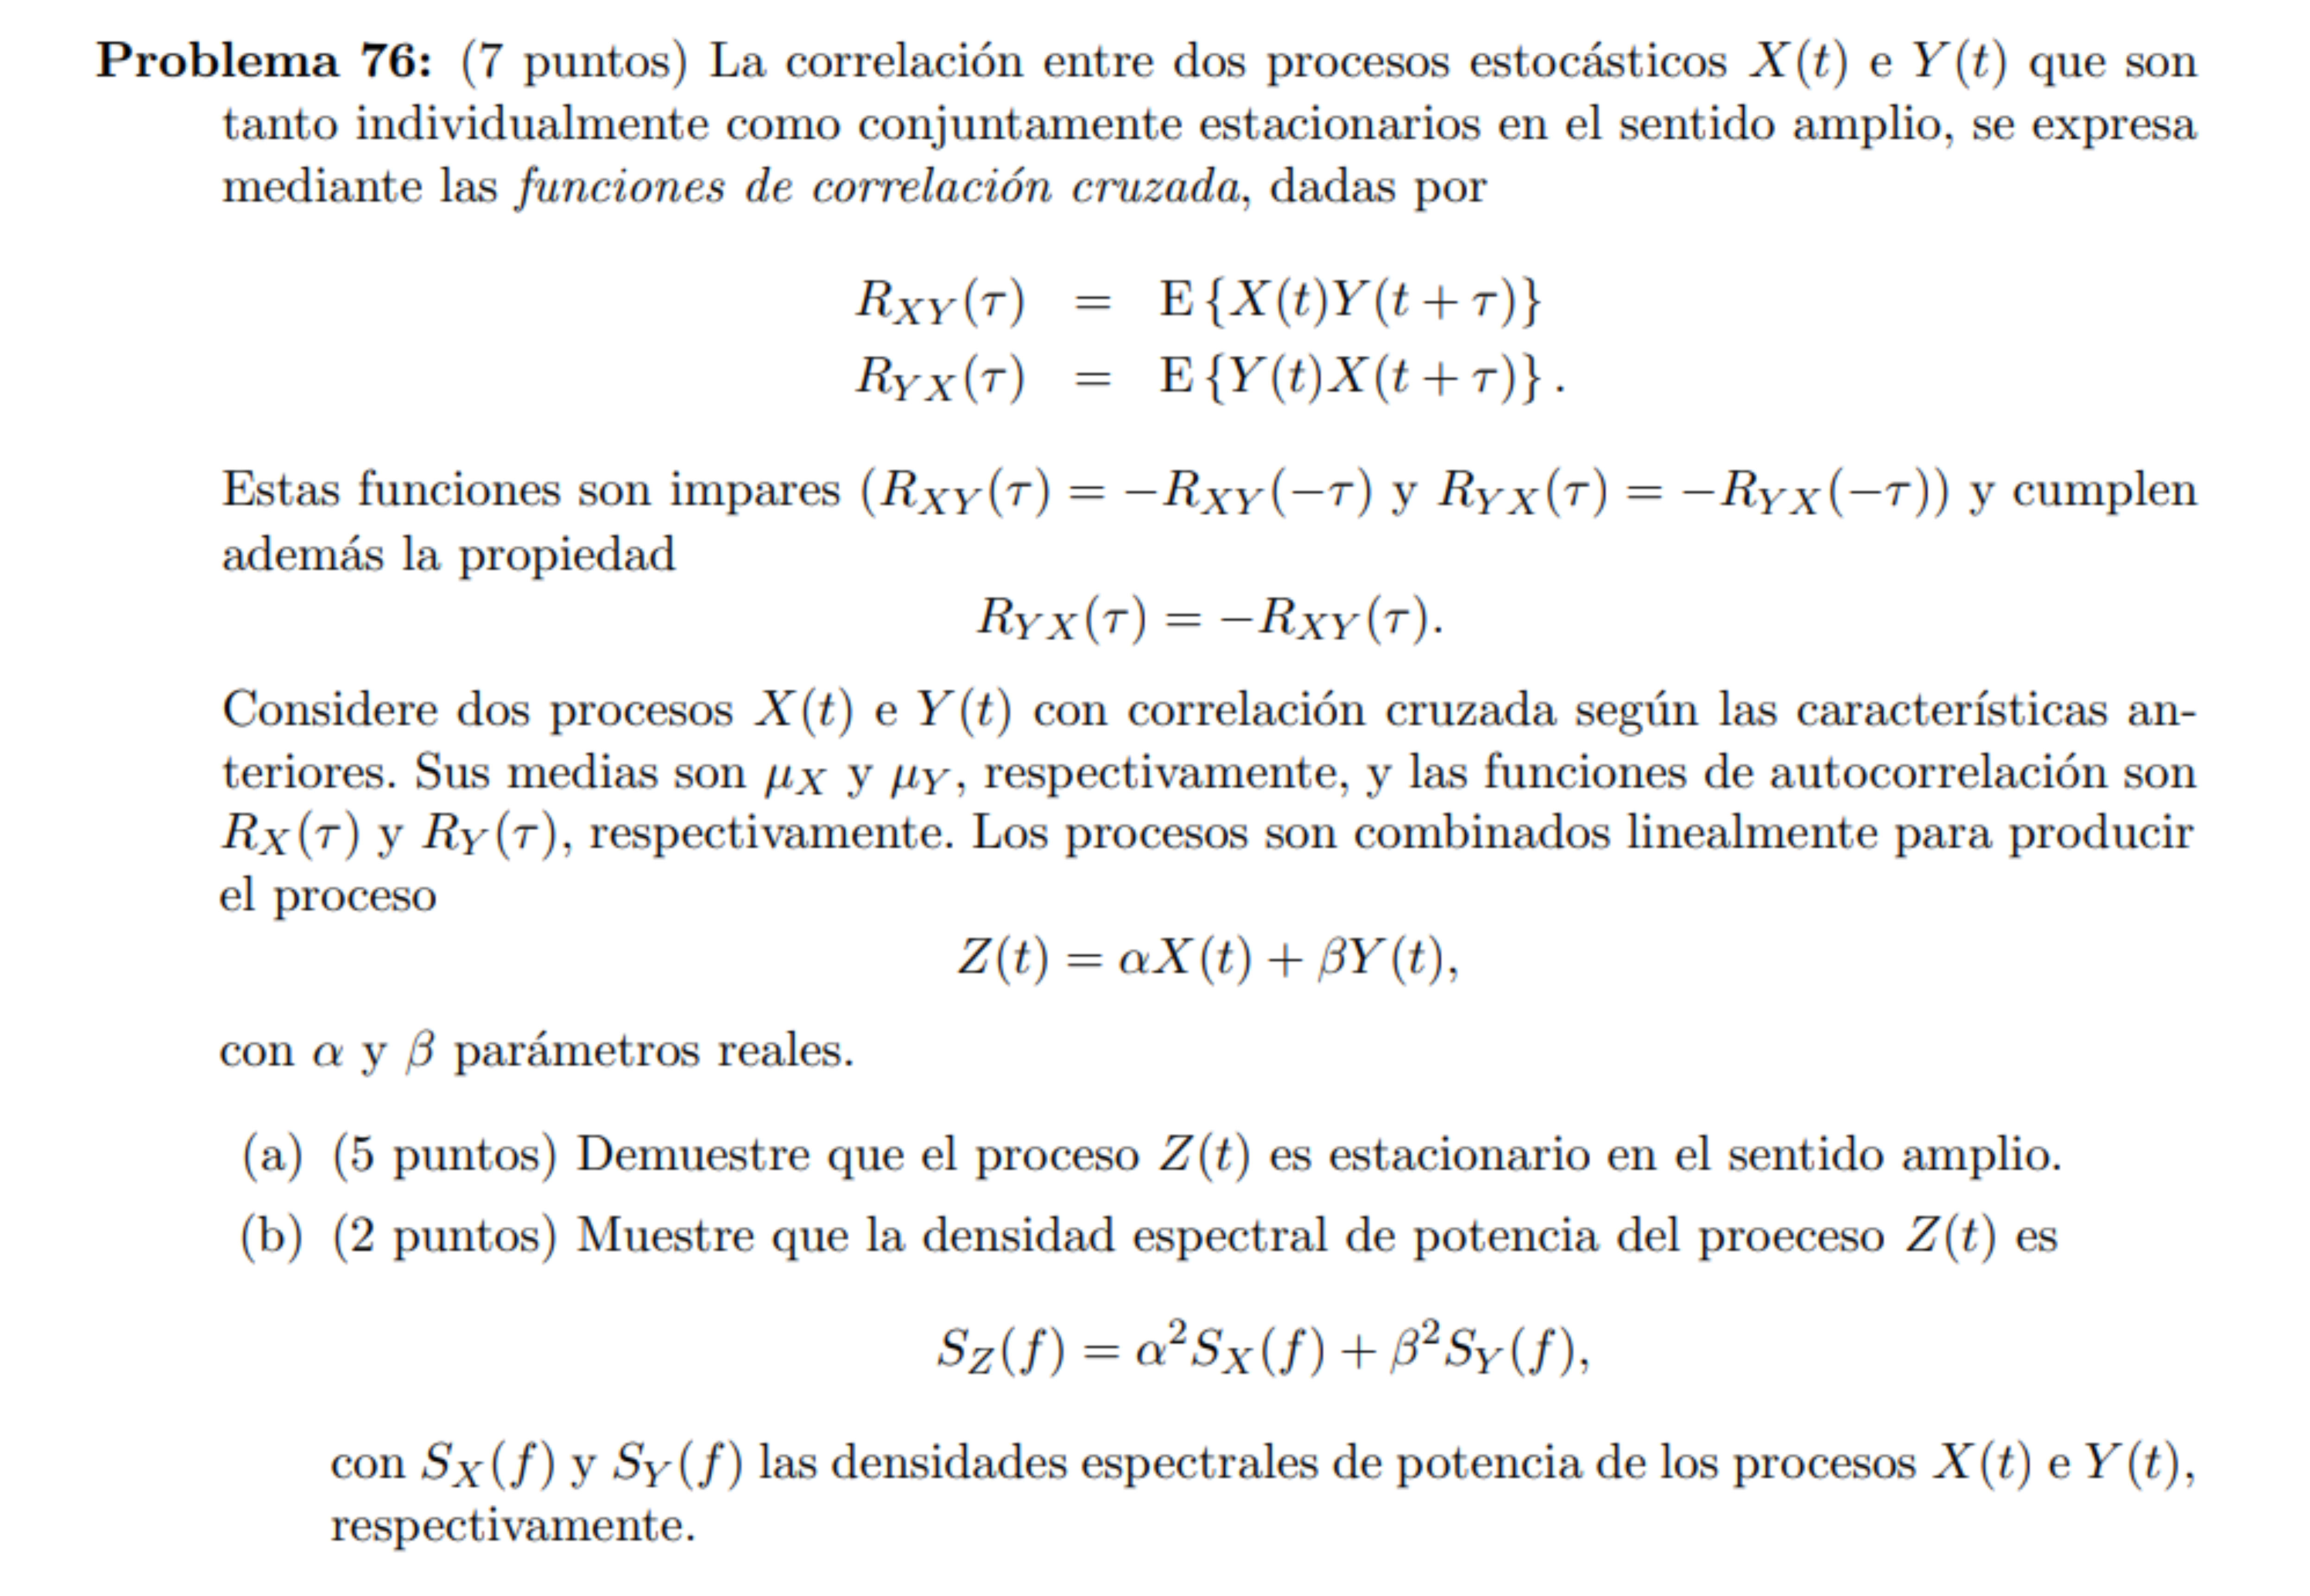
\includegraphics[width=1\textwidth]{Problema_76.png}
    \label{Problema_76}
\end{figure}
\subsection*{\small a)}
El proceso es
\[
Z(t)=\alpha X(t)+\beta Y(t)
\]
Para que sea ESA debe cumplir que:
\begin{enumerate}
    \item \(\mu_X\) sea una constante
    \item \(R(t_1,t_2)\) dependa solo de la ventana de tiempo entre \(t_1\) y \(t_2\).
\end{enumerate}

Sabemos que:
\[
\mu_Z = E[Z(t)]
\]
\[
\mu_Z = E[\alpha X(t)+\beta Y(t)]
\]
La esperanza de la suma, es la suma de las esperanzas.
\[
\mu_Z=\alpha E[X(t)]+\beta E[Y(t)]
\]
Como los procesos son estacionarios en sentido amplio
\[
E[X(t)]=\mu_X , \qquad E[Y(t)]=\mu_Y
\]
Por lo tanto
\[
\mu_Z=\alpha\mu_X+\beta\mu_Y
\]
lo cual es constante, independiente de \(t\).

Calculamos la correlacion.
\[
R_Z(\tau)=E[Z(t)Z(t+\tau)]
\]
Sustituyendo \(Z(t)\):
\[
R_Z(\tau)=E[(\alpha X(t)+\beta Y(t))(\alpha X(t+\tau)+\beta Y(t+\tau))]
\]
Expandimos:
\[
R_Z(\tau)=
\alpha^2E[X(t)X(t+\tau)]
+\beta^2E[Y(t)Y(t+\tau)]
+\alpha\beta E[X(t)Y(t+\tau)]
+\alpha\beta E[Y(t)X(t+\tau)]
\]
Usando las definiciones:
\[
R_X(\tau)=E[X(t)X(t+\tau)]
\]
\[
R_Y(\tau)=E[Y(t)Y(t+\tau)]
\]
\[
R_{XY}(\tau)=E[X(t)Y(t+\tau)]
\]
\[
R_{YX}(\tau)=E[Y(t)X(t+\tau)]
\]
Llegamos a:
\[
R_Z(\tau)=
\alpha^2 R_X(\tau)
+\beta^2 R_Y(\tau)
+\alpha\beta R_{XY}(\tau)
+\alpha\beta R_{YX}(\tau)
\]
Como el enunciado nos dice que:
\[
R_{YX}(\tau)=-R_{XY}(\tau)
\]
Entonces:
\[
\alpha \beta R_{XY}(\tau)+ \alpha \beta R_{YX}(\tau)=0
\]
Y, por lo tanto:
\[
R_Z(\tau)=\alpha^2 R_X(\tau)+\beta^2 R_Y(\tau)
\]
La funcion de autocorelacion depende solo de \(\tau\), por lo que \(Z(t)\) es estacionario en sentido amplio.

\subsection*{\small b)}
Sabemos que:
\[
S_Z(f)=\mathcal{F}\{R_Z(\tau)\}
\]
Reemplazamos:
\[
S_Z(f)=\mathcal{F}\{\alpha^2 R_X(\tau)+\beta^2 R_Y(\tau)\}
\]
Usando linealidad de la transformada de Fourier
\[
S_Z(f)=\alpha^2 \mathcal{F}\{R_X(\tau)\}+\beta^2 \mathcal{F}\{R_Y(\tau)\}
\]
\[
S_Z(f)=\alpha^2 S_X(f)+\beta^2 S_Y(f)
\]
\begin{figure}[H]
    \centering
    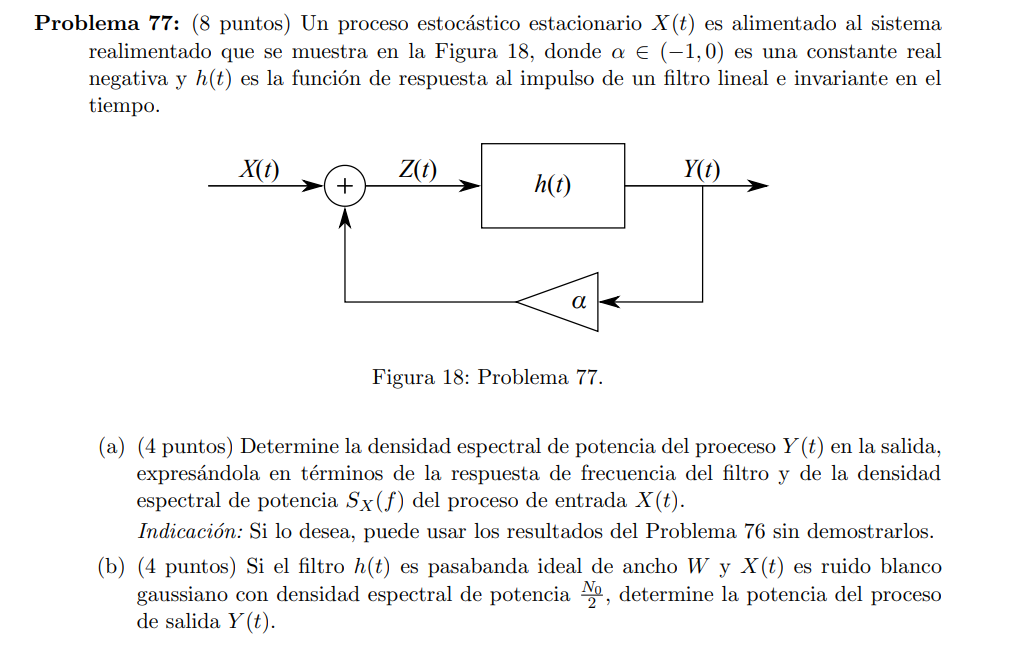
\includegraphics[width=1\textwidth]{Problema_77.png}
    \label{Problema_77}
\end{figure}
\subsection*{\small a)}
De la figura podemos definir que:
\[
Z(t)=X(t)+\alpha Y(t)
\]
Y por otro lado sabemos que como \(h(t)\) es la respuesta al impulso del sistema, entonces:
\[
Y(t)=Z(t)*h(t)
\]
Si lo analizamos en frecuencia:
\[
Y(f)=Z(f)H(f) = \left[X(f)+\alpha Y(f)\right]H(f)
\]
\[
Y(f)= X(f)H(f)+\alpha Y(f)H(f)
\]
\[
Y(f)-\alpha Y(f)H(f)= X(f)H(f)
\]
\[
Y(f)\left(1-\alpha H(f)\right)= X(f)H(f)
\]
\[
Y(f) =\left[\frac{H(f)}{\left(1-\alpha H(f)\right)}\right]X(f)
\]
De esta manera, nos queda un sistema en que entra \(Y(t)\), este pasa por un filtro y luego sale \(X(t)\). Donde el filtro corresponde a:
\[
G(f)=\frac{H(f)}{1-\alpha H(f)}
\] 
Por lo tanto:
\[
S_Y(f) = |G(f)|^{2}S_X(f)
\]
\[
S_Y(f) = \left|\frac{H(f)}{1-\alpha H(f)}\right|^{2}S_X(f)
\]
\subsection*{\small b)}
Nos dicen que ahora \(X(t)\) es ruido blanco gaussiano por lo que tiene densidad espectral:
\[
S_X(f)=\frac{N_0}{2}
\]
Y tambien nos dicen que \(h(t)\) es un filtro pasabanda ideal de ancho \(W\), es decir:
\[
H(f)=
\begin{cases}
1, & W-f_0 \le |f| \le W+f_0 \\
0, & \text{en otro caso}
\end{cases}
\]
Donde \(f_0\) es el centro de la banda pasante, se sigue entonces:
\[
|H(f)|^{2}=
\begin{cases}
1, & W-f_0 \le |f| \le W+f_0  \\
0, & \text{en otro caso}
\end{cases}
\]
De esta manera llegamos a que entonces:
\[
S_Y(f) = \left|\frac{1}{1-\alpha}\right|^{2}\frac{N_0}{2}
\]
\[
S_Y(f) = 
\begin{cases}
\frac{N_0}{2\left|1-\alpha\right|^{2}}, & W-f_0 \le |f| \le W+f_0 \\
0, & \text{en otro caso}
\end{cases}
\]
Sabemos que la potencia total de un proceso estocastico es:
\[
P_Y = \int_{-\infty}^{\infty}S_Y(f)\,df
\]
Como esta definida \(S_Y(f)\) la integral se reduce a:
\[
P_Y = 2\int_{-W+f_0 }^{W+f_0}\frac{N_0}{2\left|1-\alpha\right|^{2}}\,df
\]
Que es facil de resolver:
\[
P_Y = \frac{N_0 W}{(1-\alpha)^{2}}
\]
Como \(\alpha\in \left(-1,0\right)\) la potencia es menor que en lazo abierto.
\end{document}